\documentclass[../main.tex]{subfiles}

\begin{document}

\chapter[Topologies, Trust and Responsivity]{Topologies,\\ Trust\\ and \\Responsivity}\label{sec:topoly_trust}
\epigraph{\centering Trust is an illusion, \\M'Lady. \\I believe only in \\mutual self-interest.}
{\textit{Jupiter Ascending}\\\textsc{The Wachowskis}}


When dividing computation into different computing units, some questions are raised:
How to distribute the computation units?
Do they communicate?
How do they communicate?
In this chapter we try to answer these questions.

\minitoc

\section{How to distribute the computation units?}

The distribution of the computation units depends on the system we want to control and the processing power/number of computation units needed to solve.

For example, if the system is large but geographically in the same place, depending on the number of computation units or the processing needed, the units can be in the same hardware (here \GPU, multiple cores, threads and other strategies are used).
However, if the technical constraints (processing power) do not allow, multiple hardware must be used and a physical communication channel is needed to link the processing units.

If the system is geographically diffused and we want to use computing units to control groups of sub-systems, it is straightforward to distribute the computing units in multiple hardware placed strategically to geographically correspond to their respective groups.

For this work, we suppose that the large-scale system we want to control~\eqref{eq:large_scale_system_model} can be decomposed into geographically diffused sub-systems.
Each sub-system will have states $\vec{x}_{i}$ and inputs $\vec{u}_{i}$ that are a partition of the states and inputs of the original $\vec{x}$ and $\vec{u}$.

We suppose the optimization problem we want to use to control the system~\eqref{eq:qp_standard_form} is decomposable.
Not necessarily the computing units used to solve the sub-problems will correspond to each one of the sub-systems (Fig.~\ref{fig:noncorresponding_division_system_problem}).
For instance, a sub-problem may solve a problem with a subset of states of two different sub-systems to find the subset of inputs of a third and fourth sub-systems.

\begin{figure}[h] \centering
  \begin{subfigure}{.4\textwidth}
    \centering
    \def\svgwidth{.8\textwidth}
    \input{../img/noncorresponding_topology.pdf_tex}
    % 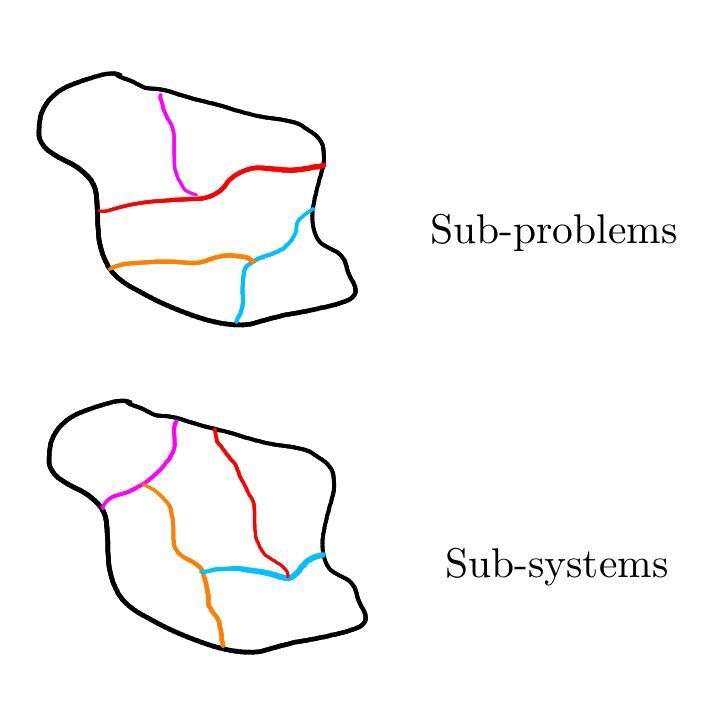
\includegraphics[width=\textwidth,clip,trim=0cm 1.8cm 0 2.5cm]{../img/noncorresponding_system_problem.png}
    \caption{Non-corresponding.}\label{fig:noncorresponding_division_system_problem}
  \end{subfigure} \hfill
  \begin{subfigure}{.4\textwidth} \centering
    \def\svgwidth{.8\textwidth}
    \input{../img/corresponding_topology.pdf_tex}
    % 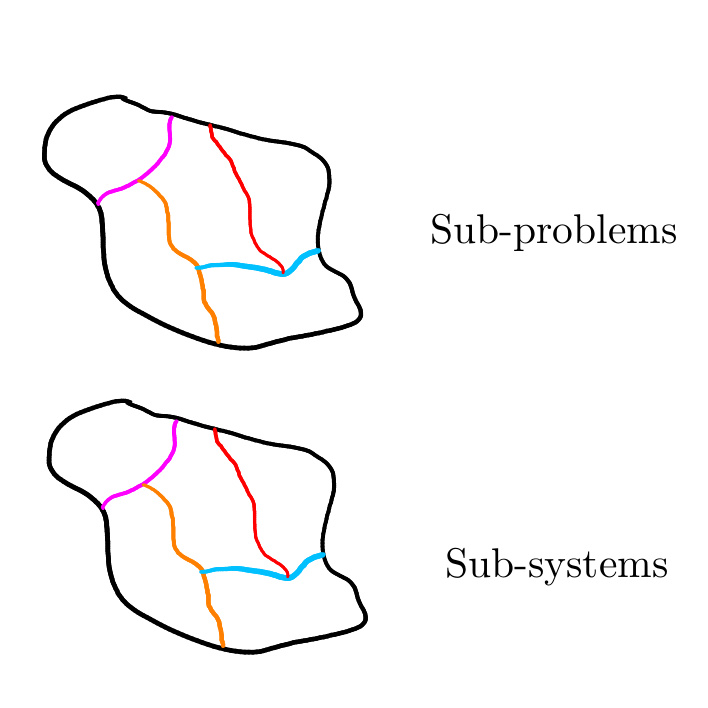
\includegraphics[width=\textwidth,clip,trim=0cm 1.8cm 0 2.5cm]{../img/corresponding_system_problem.png}
    \caption{Corresponding.}\label{fig:corresponding_division_system_problem}
  \end{subfigure}
  \caption{Decomposition of sub-problems ($P_i$) and
    sub-systems ($S_{i}$).}
\end{figure}

In the literature, it is not unusual to assume that we can choose the computing units in order to correspond to the sub-systems of the system as in Fig.~\ref{fig:corresponding_division_system_problem} (\todo[give examples of units]{Citation?}), i.e., a computing unit computes the solution of a sub-problem to find the input of the same corresponding sub-system.
So, in this work we also use this assumption.
Then, the terms sub-problems, sub-systems and agents will be used interchangeably.

\section{Do the computing units communicate?}

As shown in Section~\ref{sec:decomposable_problems}, the only case where communication is not needed to solve the optimization problem is in the uncoupled case (\S~\ref{sec:uncoupled_problems}).
However, there are some decomposition methods for the \dmpc\ that even with coupled problems, they exploit the robustness properties of the MPC to compute the solution without communication~\cite{VahidNaghaviEtAl2014}.
For the decomposition of some optimization problems, it is shown that in certain circumstances the communication is not necessary~\cite{VoulgarisElia2022}.
\begin{remark}
  Usually in \dmpc\ literature the term «decentralized» refers to frameworks where the agents do not communicate~\cite[\S 4]{ChristofidesEtAl2013},\cite{NegenbornMaestre2014}.
  The term can sometimes be confusing and be used even if the agents coordinate themselves.
  In this work we propose a different nomenclature, calling those kinds of frameworks as «uncoordinated control», since there is no coordination between agents nor a coordinator agent to referee. We use the term decentralized as opposed to centralized (monolithic), i.e. to describe structure instead of communication.
\end{remark}

The most part of the literature uses \emph{coordinated control}~\cite{NegenbornMaestre2014, ArauzEtAl2021}, in this work, analogously, we will use a decomposition method where the agents need to communicate.


\section{How do the computing units communicate?}

Multiple communication schemes exist, which depend on the decomposition, topology and also trust/power.
We can divide these schemes into two big groups (Fig.~\ref{fig:hierarchic_anarchic}), one where groups of agents are more important than others (\emph{hierarchy}), and another where there is not (\emph{anarchy}).

\begin{figure}[H]
\begin{subfigure}[b]{.45\textwidth}
  \centering
  \begin{tikzpicture}[node distance=.5cm and .5cm,inner sep=0pt,every node/.style={minimum width=0.1cm}]
    \node[draw,circle,minimum width=.7cm] at (0,0) (first) {};
    \node[draw,circle,below left=of first,minimum width=.4cm] (second_l) {};
    \node[draw,circle,below right=of first,minimum width=.4cm] (second_r) {};

    \node[draw,circle,below left =0.8cm and 0.1cm  of second_l,minimum width=.2cm] (third_1) {};
    \node[draw,circle,below right=0.8cm and -0.0cm of second_l,minimum width=.2cm] (third_2) {};
    \node[draw,circle,right      =1.8cm and 0.5cm    of third_2   ,minimum width=.2cm] (third_3) {};
    \node[draw,circle,below left =0.8cm and -0.0cm of second_r,minimum width=.2cm] (third_4) {};
    \node[draw,circle,below right=0.8cm and 0.1cm  of second_r,minimum width=.2cm] (third_5) {};

    \draw[latex-latex]  (first)  -- (second_l);
    \draw[latex-latex]  (first)  -- (second_r);
    \draw[latex-latex]  (second_l) -- (third_1);
    \draw[latex-latex]  (second_l) -- (third_2);
    \draw[latex-latex]  (second_l) -- (third_3);
    \draw[latex-latex]  (second_l) -- (third_5);
    \draw[latex-latex]  (second_r) -- (third_2);
    \draw[latex-latex]  (second_r) -- (third_3);
    \draw[latex-latex]  (second_r) -- (third_4);
    \draw[latex-latex]  (second_r) -- (third_5);
  \end{tikzpicture}
  \caption{Hierarchy.}\label{fig:hierarchy_topology}
\end{subfigure}
\hfill
\begin{subfigure}[b]{.45\textwidth}
  \centering
  \begin{tikzpicture}[node distance=.5cm and .5cm,inner sep=0pt,every node/.style={minimum width=0.3cm}]
    \node[draw,circle] at (0,0) (a) {};
    \node[draw,circle] at ($(a)+(-.7,-.3)$) (b) {};
    \node[draw,circle] at ($(a)+(0.0,-0.8)$) (c) {};
    \node[draw,circle] at ($(a)+(0.8,-0.4)$) (d) {};
    \node[draw,circle] at ($(b)+(0.1,-1.0)$) (e) {};
    \node[draw,circle] at ($(e)+(1.2,-0.1)$) (f) {};
    \node[draw,circle] at ($(f)+(0.6,0.4)$) (g) {};
    \node[draw,circle] at ($(e)+(-0.8,-0.0)$) (h) {};
    \node[draw,circle] at ($(f)+(-0.5,-0.5)$) (i) {};

    \draw[latex-latex]  (a)  -- (b);
    \draw[latex-latex]  (a)  -- (c);
    \draw[latex-latex]  (a)  -- (d);
    \draw[latex-latex]  (b)  -- (c);
    \draw[latex-latex]  (c)  -- (d);
    \draw[latex-latex]  (e)  -- (b);
    \draw[latex-latex]  (e)  -- (c);
    \draw[latex-latex]  (c)  -- (f);
    \draw[latex-latex]  (d)  -- (g);
    \draw[latex-latex]  (f)  -- (g);
    \draw[latex-latex]  (e)  -- (h);
    \draw[latex-latex]  (f)  -- (i);
  \end{tikzpicture}
  \caption{Anarchy}\label{fig:anarchy_topology}
\end{subfigure}
\caption{Hierarchic and anarchic topologies.\todo[redo figures, add stages to identify power]{}}\label{fig:hierarchic_anarchic}
\end{figure}


Sometimes the hierarchical structure may be implied by the decomposition. For instance, some decompositions (\todo[exemplos de sequential dado em ChristofidesEtAl2013]{Citation?}) need the agents to solve their problems one after the other until the values converge (Fig.~\ref{fig:sequential_topology}).
These schemes are called \emph{sequential}.
We can see a hierarchy among the agents, since although a convergence is reached, one group of agents solve their problems disregard the others, giving them an initial position of power, even if temporary.
In other decompositions (\todo[exemplos de parallel dado em ChristofidesEtAl2013]{Citation?}), all agents solve their problems independently of others and then share results until convergence is reached, iteratively or not (Fig.~\ref{fig:parallel_topology}).
These structures are called \emph{parallel}.
In such structures there is no hierarchy.


\begin{figure}[h]
\begin{subfigure}[b]{.45\textwidth}
  \centering
  \begin{tikzpicture}[node distance=1cm and .5cm]
    \node[draw,circle] (first) at (0,0) {};
    \node[draw,circle,right=of first] (second) {};
    \node[draw,circle,right=of second] (third) {};
    \node[draw,circle,opacity=0,right=of third] (fourth) {};
    \node[draw,circle,right=of fourth] (fifth) {};

    \node[] at (fourth) {...};
    \draw[-latex] (first) -- (second);
    \draw[-latex] (second) -- (third);
    \draw[-latex] (third) -- (fourth);
    \draw[-latex] (fourth) -- (fifth);
  \end{tikzpicture}
  \caption{Sequential topology.}\label{fig:sequential_topology}
\end{subfigure}
\hfill
\begin{subfigure}[b]{.45\textwidth}
  \centering
  % 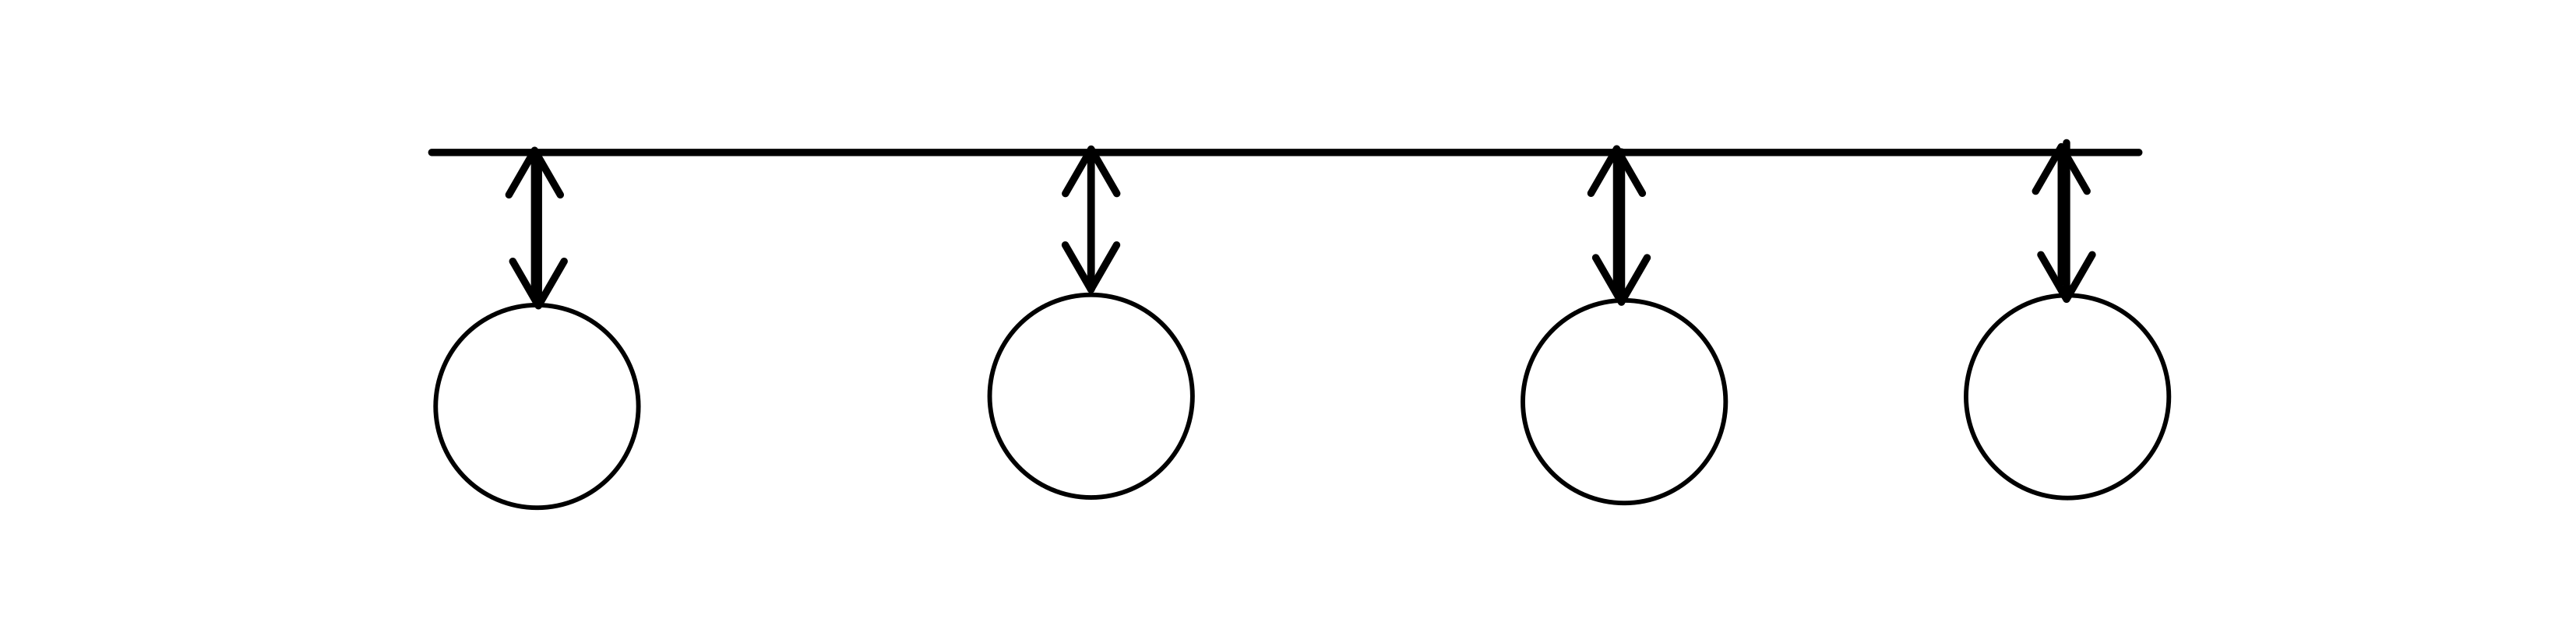
\includegraphics[width=\textwidth]{../img/parallel_topology.png}
  \begin{tikzpicture}[node distance=.5cm and .5cm,inner sep=0pt,minimum width=.5cm]
    \node[draw,rectangle,fill=black,minimum height=2pt,minimum width=5cm] (bar) at (0,0) {};
    % \draw[blue,fill] ($(bar)+(-2.5cm,-2pt)$) rectangle ($(bar)+(2.5cm,2pt)$);
    \node[draw,circle,below=of bar] (third) {};
    \node[draw,circle,left=of third] (second) {};
    \node[draw,circle,left=of second] (first) {};
    \node[draw,circle,opacity=0,right=of third] (fourth) {};
    \node[draw,circle,right=of fourth] (fifth) {};

    \node[] at (fourth) {...};
    \draw[latex-latex]  (first)  -- (bar.south -| first);
    \draw[latex-latex]  (second) -- (bar.south -| second);
    \draw[latex-latex]  (third)  -- (bar.south -| third);
    \draw[latex-latex]  (fifth)  -- (bar.south -| fifth);
  \end{tikzpicture}
  \caption{Parallel topology.}\label{fig:parallel_topology}
\end{subfigure}
\caption{Sequential and parallel topologies.}\label{fig:sequential_parallel_topology}
\end{figure}

And in other decompositions the hierarchical structure can be chosen.
For example, when negotiation between agents is needed, questions about trust and security can shape the presence or absence of hierarchy.
One of these questions is: Can an agent trust all other agents?

This question is common in multiple areas where communication, exchanges or consensus between a large number of agents are needed (politics, economy, and others).
If an agent distrusts the others, it can treat itself the security issues or the agent can outsource the treatment to another agent.
Additional agents can be included to serve as referees, coordinators, regulators or certifiers. It is done because it is easier to trust in/verify a single agent or small group of agents than to trust in all agents. This way the work is divided into more manageable parts.

One real life example can be the \EFT\ between a seller and client. A seller instead of trusting the credit (capacity of paying in future date) of each of its clients, she or he trusts in a small group of credit card brands to fulfill the \EFT{}.
Each credit card brand, in turn, trusts in a select group of credit-granting institutions, to which potentially these client are associated.
This kind of arrangement creates a hierarchical tree-like structure called \emph{polytree} in graph theory terms (Fig.~\ref{fig:polytree_topology}). Seller and clients are leafs (terminal nodes), credit card-brands are branch vertex (intermediary) and the credit-granting institutions are roots (no parent nodes).
Some other political/societal parallel views are stablished in~\cite{McNamaraEtAl2018} and~\cite{OlaruEtAl2018}.
\begin{figure}[h]
  \centering
  \begin{tikzpicture}[every node/.style={circle,draw,minimum width=0.5cm},inner sep=0pt,node distance=1.cm and 0.5cm]
    \node[] (a) at (0,0) {};
    \node[right=of a] (b)  {};
    \node[right=of b] (c)  {};
    \node[right=of c] (d)  {};

    \node[below right=of a] (e)  {};
    \node[right      =of e] (f)  {};
    \node[right      =of f] (g)  {};

    \node[minimum width=0.2cm,below left=1.0cm and .5cm of e] (h)  {};
    \node[minimum width=0.2cm,right     =of h] (i)  {};
    \node[minimum width=0.2cm,right     =of i] (j)  {};
    \node[minimum width=0.2cm,right     =of j] (k)  {};
    \node[minimum width=0.2cm,right     =of k] (l)  {};
    \node[minimum width=0.2cm,right     =of l] (m)  {};

    \draw[-latex] (a) -- (e);
    \draw[-latex] (a) -- (g);
    \draw[-latex] (b) -- (e);
    \draw[-latex] (b) -- (f);
    \draw[-latex] (c) -- (e);
    \draw[-latex] (c) -- (f);
    \draw[-latex] (c) -- (g);
    \draw[-latex] (d) -- (g);
    \draw[-latex] (e) -- (h);
    \draw[-latex] (e) -- (i);
    \draw[-latex] (e) -- (j);
    \draw[-latex] (e) -- (l);
    \draw[-latex] (f) -- (i);
    \draw[-latex] (f) -- (j);
    \draw[-latex] (f) -- (k);
    \draw[-latex] (f) -- (l);
    \draw[-latex] (g) -- (m);
  \end{tikzpicture}
  \caption{A polytree.}\label{fig:polytree_topology}
\end{figure}

\subsection{Some drawbacks and compromises}\label{sec:drawbacks}

\paragraph{Failure}
Although the hierarchical structure can help reducing the sources of distrust, it also reduce responsitivity and robustness.
If a small number of the intermediary or most highly nodes in the hierarchical tree are inoperative, there is a possibility that the complete system collapses since the communications will not be accomplished, this problem is commonly known as the \emph{single point of failure}, which can be deviated by the use of redundancy.
On the other hand, for non-hierarchical structures, the system only perish if the majority of the nodes is inoperative or compromised.

\paragraph{Energy consumption and Environment}
To overcome the problem of trust in anarchic (peer-to-peer) structures, a solution recently in vogue called \emph{blockchain} was proposed~\cite{Nakamoto2008}.
% The strategy targets exchange of validable data that dependend on historic data.
In this solution, all historic data (log) are shared between all agents.
Before beeing sent to all other agents (or only neighbours), new data need to be processed to generate a \emph{proof of work} (proof of a difficult computation which is easy to test) to create a block.
This block needs to be validated (data and \emph{proof of work} are valid) by at least more than half of the agents before beeing chained into the historic data, forming a chain of blocks, thus the name.

As each block has a different \emph{proof of work}, to create an new block with unreasonable data, an ill-intentioned agent needs to alter all the past blocks in the chain recreating all \emph{proofs of work} one by one, until the false data could be accepted.
This way, the attacker would need to have more than half of the total processing power of the network.
The \emph{proof of work} strategy trades trust by energy.
A recent work~\cite{ColeCheng2018} estimates the energy consumption of one of the most diffused application of the \emph{blockchain}, a crypto-currency called Bitcoin.
It estimates that each transaction consumes at least $200$kWh, which is greater than the monthly electrical consumption of a small household of two people in Brazil~\cite{EPE2022}.
A more recent work~\cite{RoeckDrennen2022} makes a Life Cycle Assessment of Bitcoin mining in a power plant and concludes that its annual emissions of metric tons of CO$_2$-eq is comparable to the annual emissions of 140,000 passenger vehicles.

% \subsection{Conclusion}
All the points above and many others must be considered before choosing a structure.
\todo[some??]{Some} works in the literature of \dmpc\ \cite{VelardeEtAl2017a, BoemEtAl2020, LiuEtAl2022} use an anarchic structure.
Although some methods shown in this work could be adapted to function in analogous structures, we opt to use the hierarchical approach instead. We add coordinator(s) which referee the exchange between agents.

% \chapterEndOrnament

\printbibliography
\end{document}
